\documentclass[a4paper,11pt]{article}

% ------------------------------
% Geometry and Page Layout
% ------------------------------
\usepackage{geometry}
\geometry{left=1in, right=1in, top=1in, bottom=1in} % Set 1-inch margins
\usepackage{fancyhdr}   % Header and footer customization
\usepackage{pdflscape}  % Landscape pages
\usepackage{everypage}  % Add hooks to every page

% ------------------------------
% Font and Typography
% ------------------------------
\usepackage{mathptmx}   % Use Times New Roman font (or Computer Modern by default)
\renewcommand{\baselinestretch}{1.5} % Line spacing
\usepackage[utf8]{inputenc} % UTF-8 support
\usepackage{tocloft}
\usepackage[normalem]{ulem}

% ------------------------------
% For customizing titles
% ------------------------------
\usepackage{titlesec}
% Redefine \section to be unnumbered but still included in TOC
\titleformat{\section}[hang]{\centering\normalfont\Large\bfseries}{}{0pt}{} % Removes numbering from section titles

% ------------------------------
% Date Handling
% ------------------------------
\usepackage[english]{datetime2}
\DTMnewdatestyle{mydateA}{%
  \renewcommand*{\DTMdisplaydate}[4]{%
    \DTMtwodigits{##3}/\DTMtwodigits{##2}/##1}%
  \renewcommand*{\DTMDisplaydate}{\DTMdisplaydate}%
}
\DTMnewdatestyle{mydateB}{%
  \renewcommand*{\DTMdisplaydate}[4]{%
    \DTMtwodigits{##3} \DTMenglishmonthname{##2} ##1}%
  \renewcommand*{\DTMDisplaydate}{\DTMdisplaydate}%
}

% ------------------------------
% Color and Graphics
% ------------------------------
\usepackage[table]{xcolor}
\definecolor{mygreen}{rgb}{0.82, 0.94, 0.75}
\definecolor{mygreen2}{rgb}{0.67, 0.88, 0.69}
\definecolor{codegreen}{rgb}{0,0.94,0}
\definecolor{codegray}{rgb}{0.5,0.5,0.5}
\definecolor{codepurple}{rgb}{0.58,0,0.82}
\definecolor{backcolour}{rgb}{0.95,0.95,0.92}
\usepackage{graphicx}   % For including figures
\graphicspath{{}}       % Set graphic paths
\DeclareGraphicsExtensions{.pdf,.jpeg,.png,.jpg}
\usepackage{tikz}       % For custom drawings and diagrams
\usepackage{subcaption}  % For subfigures
\usepackage{float}

% ------------------------------
% Mathematics
% ------------------------------
\usepackage{amsmath}    % Mathematical symbols and environments
\usepackage{amssymb}    % Additional math symbols
\usepackage{yhmath}     % Extended math fonts
\usepackage{extarrows}  % Extensible arrows
\usepackage{esint}      % Integrals
\usepackage{bigints}    % Large integral symbols
\usepackage{mathrsfs}   % Script math font

% ------------------------------
% Code Formatting
% ------------------------------
\usepackage{listings}   % Code listings
\lstdefinestyle{mystyle}{
    backgroundcolor=\color{backcolour},   
    commentstyle=\color{green!50!black},
    keywordstyle=\color{blue},
    numberstyle=\tiny\color{codegray},
    stringstyle=\color{red},
    basicstyle=\ttfamily\footnotesize, % Adjusting the code size here
    breakatwhitespace=false,         
    breaklines=true,                 
    captionpos=b,                    
    keepspaces=true,                 
    numbers=left,                    
    numbersep=5pt,                  
    showspaces=false,                
    showstringspaces=false,
    showtabs=false,                  
    tabsize=2,
    frame=single,
    captionpos=b
}
\lstset{style=mystyle}

% ------------------------------
% Bibliography Management
% ------------------------------
\usepackage[
            backend=biber, 
            isbn=false, 
            url=true, 
            doi=true, 
            giveninits=true, 
            sorting=nyt]{biblatex}
\addbibresource{ref.bib}

% Optional: Customize title formatting to keep hyperlinks intact
\newbibmacro{string+doi}[1]{%
  \iffieldundef{doi}{#1}
  {\href{https://doi.org/\thefield{doi}}{#1}}}

\DeclareFieldFormat{title}{\usebibmacro{string+doi}{\mkbibemph{#1}}}
\DeclareFieldFormat[article]{title}{\usebibmacro{string+doi}{\mkbibquote{#1}}}
\DeclareFieldFormat[article,periodical]{volume}{\mkbibbold{#1}}
\DeclareFieldFormat[article,periodical]{number}{\mkbibbold{#1}}

% ------------------------------
% Packages for Tables
% ------------------------------
\usepackage{array}      % Extended column definitions
\usepackage{tabularx}   % Table with adjustable-width columns
\usepackage{longtable}  % Tables spanning multiple pages
\usepackage{booktabs}   % Formal tables
\usepackage{arydshln}   % Dashed lines in tables
\usepackage{multirow}   % Multi-row cells
\usepackage{makecell}   % Enhanced table cells
\usepackage{tasks}      % Task lists within tables
\usepackage{adjustbox}
% ------------------------------
% Custom Commands and Settings
% ------------------------------
\newcommand{\checkbox}{\makebox[0.5cm]{\strut $\square$}} % Custom checkbox command
\newcommand{\RotatePagenumber}{%
  \ifdim\textwidth=\linewidth
    % Do nothing if text width equals line width
  \else
    \begingroup
    \dimendef\margins=0
    \ifodd\value{page}
      \margins=\oddsidemargin
    \else
      \margins=\evensidemargin
    \fi
    \raisebox{\dimexpr -\topmargin-\headheight-\headsep-\footskip-1cm}[0pt][0pt]{%
      \rlap{\hspace{\dimexpr \margins + \textheight + \footskip + \marginparwidth}%
      \llap{\rotatebox{90}{\thepage}}}}%
    \endgroup
  \fi
}
\AddEverypageHook{\RotatePagenumber} % Apply custom page numbering

% ------------------------------
% Color and Hyperlink Settings
% ------------------------------
\usepackage[colorlinks]{hyperref}
\hypersetup{
    linkcolor=blue,   % Color for internal links
    citecolor=red,    % Color for citations
    urlcolor=purple,  % Color for URLs
}

% ------------------------------
% cross reference
% ------------------------------
\usepackage[nameinlink,capitalize]{cleveref} %cross reference showing Eq. (1) etc.

% ------------------------------
% Start Document
% ------------------------------
\begin{document}
\thispagestyle{empty}
\DTMsetdatestyle{mydateA}

%%%%%%%%%%%%%%%%%%%%%%%%%%%%%%%%%%%%%%%%%%%%%%%%%%%%%%%%%%%%%%%%%%%%%%%%%%%%%%%%%%%%%%%%
% Slip
%%%%%%%%%%%%%%%%%%%%%%%%%%%%%%%%%%%%%%%%%%%%%%%%%%%%%%%%%%%%%%%%%%%%%%%%%%%%%%%%%%%%%%%%
%SCHOOL OF PHYSICS -- LEVEL 200 PHYSICS LABORATORY REPORT SLIP
\begin{center}
    \textbf{SCHOOL OF PHYSICS -- LEVEL 200 PHYSICS LABORATORY REPORT SLIP} \\
    \textbf{FOR ZCT 293/2 AND ZCT 294/2}
\end{center}

\begin{table}[h]
\begin{center}
\resizebox{\textwidth}{!}{
\begin{tabular}{|llllllllllllllllllll|}
\hline
\multicolumn{20}{|l|}{\textbf{Instructions to student:} Please make sure you fill in the form completely.} \\
\multicolumn{20}{|l|}{\textbf{Instructions to lecturer:} Kindly record the numerical marks in the rubric assessment form, not here.} \\ \hline
\multicolumn{20}{|c|}{
  \centering{\textbf{PARTICULARS}}
}                                                                                                                                      \\ \hline
Name & :\,\,TAN WEI LIANG & \multicolumn{18}{l|}{}                                                                                                                                                                        
\\ \hline
Matric no. & :\,\,22302889  & \multicolumn{18}{l|}{}                                                                                                                                                                        
\\ \hline
Group& :\,\,W2  & \multicolumn{18}{l|}{}                                                                                                                                                                        
\\ \hline
Expt. Code & :\,\,2OS3 & \multicolumn{18}{l|}{}                                                                                                                                                                        
\\ \hline
Expt. Title & :\,\,MICHELSON INTERFEROMETER & \multicolumn{18}{l|}{}                                                                                                                                                                        
\\ \hline
Lecturer in charge & :\,\,DR. AFIQ ARIF AMINUDDIN JAFRY & \multicolumn{18}{l|}{}                                                                                                                                                                        
\\ \hline
Report due date & :\,\,22/1/2025 & \multicolumn{18}{l|}{}                                                                                                                                                                        
\\ \hline
\multicolumn{11}{|c|}{\textbf{Experiment (\checkmark)}} & \multicolumn{9}{c|}{\textbf{Lab Report Grade (\checkmark)}} \\ 
\hline
\multicolumn{11}{|c|}{1 $\square$ \quad 2 $\square$ \quad 3 $\square$ \quad 4 $\square$ \quad 5 $\square$ \quad 6 $\text{\rlap{$\checkmark$}}\square$} & 

\multicolumn{1}{l|}{A} & \multicolumn{1}{l|}{$\square$} &
\multicolumn{1}{l|}{A$-$} & \multicolumn{1}{l|}{$\square$} &
\multicolumn{1}{l|}{B$+$} & \multicolumn{1}{l|}{$\square$} &
\multicolumn{1}{l|}{B} & \multicolumn{1}{l|}{$\square$} 
&\multicolumn{1}{l|}{}
\\ \hline
\multicolumn{11}{|l|}{} & 

\multicolumn{1}{l|}{B$-$} & \multicolumn{1}{l|}{$\square$} &
\multicolumn{1}{l|}{C$+$} & \multicolumn{1}{l|}{$\square$} &
\multicolumn{1}{l|}{C} & \multicolumn{1}{l|}{$\square$} &
\multicolumn{1}{l|}{C$-$} & \multicolumn{1}{l|}{$\square$} 
&\multicolumn{1}{l|}{}
\\ \hline

\multicolumn{11}{|c|}{} & 

\multicolumn{1}{l|}{D$+$} & \multicolumn{1}{l|}{$\square$} &
\multicolumn{1}{l|}{D} & \multicolumn{1}{l|}{$\square$} &
\multicolumn{1}{l|}{D$-$} & \multicolumn{1}{l|}{$\square$} &
\multicolumn{1}{l|}{F} & \multicolumn{1}{l|}{$\square$} 
&\multicolumn{1}{l|}{}
\\ \hline
\multicolumn{20}{|c|}{} \\\hline 
\multicolumn{10}{|c|}{Date Received (Stamp):} & 
\multicolumn{10}{c|}{Comments:}  \\ \hline   
\multicolumn{10}{|c|}{} & 
\multicolumn{10}{c|}{}\\
\multicolumn{10}{|c|}{} & 
\multicolumn{10}{c|}{}\\
\multicolumn{10}{|c|}{} & 
\multicolumn{10}{c|}{}\\
\multicolumn{10}{|c|}{} & 
\multicolumn{10}{c|}{}\\
\multicolumn{10}{|c|}{} & 
\multicolumn{10}{c|}{}\\
\multicolumn{10}{|c|}{} & 
\multicolumn{10}{c|}{}\\\hline     
\end{tabular}
}
\end{center}
\end{table}

\newpage

\thispagestyle{empty}

\begin{center}
\textbf {\Large REPORT SUBMISSION FORM}
\end{center}

\begin{figure}[ht]
\begin{flushright}

\includegraphics[width=0.28\textwidth]{USMlogo}
\end{flushright}
\end{figure}

\large
\begin{tabular}{lcl}
Name & : &\dotuline{TAN WEi LIANG\hfill}\\
\\
Partner's Name &: &\dotuline{TAN SHUENN PYNG\hfill}\\
\\
Group& : &\dotuline{W2\hfill}\\
\\
Experiment Code& :&\dotuline{2OS3\hfill}\\
\\
Experiment Title&: &\dotuline{MICHELSON INTERFEROMETER\hfill}\\
\\
Lecturer's/Examiner's&: &\dotuline{DR. AFIQ ARIF AMINUDDIN JAFRY\hfill}\\ 
Name\\
\\
Starting Date &: &\dotuline{8/1/2025\hfill}\\
(1st session)\\
\\
Ending Date &: &\dotuline{15/1/2025\hfill}\\
(2nd session)\\
\\
Submission Date &: &\dotuline{$\today$\hfill}\\
\\
\end{tabular}


\newpage
\thispagestyle{empty}

\begin{center}
\textbf{\Large DECLARATION OF ORIGINALITY}
\end{center}
\bigskip
I, \textbf{TAN WEI LIANG 22302889}
hereby declare that this laboratory report is my own work. I further declare that:

\begin{enumerate}
    \item The references/bibliography reflect the sources I have consulted, and
    \item I also certify that this report has not previously been submitted for assessment in this or any other units, and that I have not copied in part or whole or otherwise plagiarized the work of other students and/or persons.
    \item Sections with no source referrals are my own ideas, arguments, and/or conclusions.
\end{enumerate}

\bigskip
\begin{figure}[htbp]
\hspace{35mm}
\includegraphics[width=0.1\linewidth]{signature}
\label{6}
\vspace{-12mm}
\end{figure}
\noindent Signature: \hrulefill \hfill Date: \uline{$\today$}

\newpage

%%%%%%%%%%%%%%%%%%%%%%%%%%%%%%%%%%%%%%%%%%%%%%%%%%%%%%%%%%%%%%%%%%%%%%%%%%%%%%%%%%%%%%%%%%%
%Reporty Content
%%%%%%%%%%%%%%%%%%%%%%%%%%%%%%%%%%%%%%%%%%%%%%%%%%%%%%%%%%%%%%%%%%%%%%%%%%%%%%%%%%%%%%%%%%%
\thispagestyle{empty}

\DTMsetdatestyle{mydateB}

%%%
\begin{center}
\vspace*{1cm}
\textbf{\Large MICHELSON INTERFEROMETER}

\vspace{3.0cm}
\textbf{\Large By}\\

\vspace{3.0cm}
\textbf{\Large TAN WEI LIANG} \\

\vspace{6.0cm}
\textbf{\Large \today}\\

\vfill
\textbf{\Large Second Year Laboratory Report}
\end{center}
\newpage

%%%
\pagenumbering{roman}
\phantomsection
\section*{\Large \center MICHELSON INTERFEROMETER}
\addcontentsline{toc}{section}{ABSTRACT}
\section*{\large \center ABSTRACT}
\label{sec:ABSTRACT}

\qquad The title of this experiment is \textbf{MICHELSON INTERFEROMETER}. In this experiment, the focus was determine the wavelength and coherence length of a He-Ne laser. The setup was meticulously aligned to produce interference patterns, allowing precise determination of the laser's wavelength by varying the optical path difference using a micrometer screw while counting interference fringes. The measured wavelength, averaging 633.97 nm, showed excellent agreement with the theoretical value of 632.8 nm, demonstrating a minimal discrepancy of 0.18\%. Additionally, the coherence length was assessed through the contrast function derived from photodiode intensity measurements, with a measured value of 9.16 cm closely matching the theoretical prediction of 8.86 cm, yielding a percentage difference of 3.33\%. These findings highlight the effectiveness of the Michelson Interferometer in precision optical measurements and its relevance in exploring coherence and interference phenomena.


\newpage 
%%%%%%%%%%%%%%%%%%%%%%%%%%%%%%%%%%%%%%%%
\phantomsection
\addcontentsline{toc}{section}{ACKNOWLEDGEMENTS}
\section*{\large \center ACKNOWLEDGEMENTS}
\label{sec:ACKNOWLEDGEMENTS}

\qquad First and foremost, I express my sincere appreciation to DR. AFIQ ARIF AMINUDDIN JAFRY, our distinguished lecturer and examiner, for the invaluable guidance and unwavering support extended throughout our scientific exploration. I extend my sincere gratitude to my experiment partner, TAN SHUENN PYNG. His invaluable cooperation and dedication throughout both experiments were instrumental to the success of this project. I appreciate his commitment, expertise, and teamwork, which made these scientific endeavours both productive and enjoyable.

\newpage
%%%%%%%%%%%%%%%%%%%%%%%%%%%%%%%%%%%%%%%%%
\renewcommand{\contentsname}{CONTENTS}
\renewcommand{\cftsecleader}{\cftdotfill{\cftdotsep}} % Ensures dotted lines for sections
% Adjust the dot separation
\renewcommand{\cftdotsep}{1.0} % Default is 4.5, decrease for more dots
\begin{center}
\tableofcontents
\end{center}
\label{sec:CONTENTS}

\newpage
%%%%%%%%%%%%%%%%%%%%%%%%%%%%%%%%%%%%%%%%%
\renewcommand{\listtablename}{LIST OF TABLES}
\phantomsection
\addcontentsline{toc}{section}{LIST OF TABLES}
\label{sec:LIST OF TABLES}
\begin{center}
\listoftables
\end{center}

\newpage
%%%%%%%%%%%%%%%%%%%%%%%%%%%%%%%%%%%%%%%%%
\renewcommand{\listfigurename}{LIST OF FIGURES}
\phantomsection
\addcontentsline{toc}{section}{LIST OF FIGURES}
\label{sec:LIST OF FIGURES}
\begin{center}
\listoffigures
\end{center}

\newpage
%%%%%%%%%%%%%%%%%%%%%%%%%%%%%%%%%%%%%%%%%
\phantomsection
\pagenumbering{arabic} 
\section{\centering INTRODUCTION}
\label{sec:INTRODUCTION}

\indent

The Michelson Interferometer, invented by Albert A. Michelson in the late 19th century, is a fundamental instrument in optical physics, renowned for its precision in measuring wavelengths, small distances, and refractive indices. It operates by splitting a beam of light into two paths, reflecting them back, and recombining them to produce interference patterns. These patterns are highly sensitive to changes in optical path lengths, making the interferometer a powerful tool for various applications, including the historical Michelson-Morley experiment, which provided critical evidence against the existence of the luminiferous aether and paved the way for the development of the theory of relativity \cite{michelson_morley_1887}.




\newpage
%%%%%%%%%%%%%%%%%%%%%%%%%%%%%%%%%%%%%%%%%
\phantomsection
\section{\centering THEORY}
\label{sec:THEORY}
% Theory Part
\indent

\subsection{Michelson Interferometer}
\indent

The interferometer splits a beam of light into two perpendicular paths using a beam splitter. The beams reflect off mirrors \(M_1\) and \(M_2\) and recombine at the beam splitter to produce interference patterns. These patterns arise due to variations in the optical path difference (\(\Delta L\)) between the two arms. The path difference is given by:
\[
\Delta L = 2d \cos \theta,
\]
where \(d\) is the distance to the mirror and \(\theta\) is the angle of incidence. For a collimated beam (\(\theta \approx 0\)), the equation simplifies to \(\Delta L = 2d\).\\

The resulting interference pattern consists of circular fringes, where each successive bright fringe corresponds to a path difference equal to an integer multiple of the wavelength (\(\lambda\)):
\[
2\Delta d = n\lambda,
\]
with \(n\) as the fringe order. These circular fringes are a hallmark of the Michelson Interferometer and provide a mechanism for precise measurements.\\

\subsection{Temporal Coherence and Coherence Length \autocite{phywe_2019}\autocite{UCSB_HeNe_Lasers}}
\indent

Temporal coherence characterizes the ability of light waves to maintain phase correlation over time. It is directly tied to the coherence length (\(L_{\text{coh}}\)), which represents the maximum optical path difference over which interference remains observable. The coherence length is inversely proportional to the spectral bandwidth (\(\Delta \nu\)) of the light source:
\[
L_{\text{coh}} = \frac{c}{\Delta \nu},
\]
where \(c\) is the speed of light.

For narrowband sources like the He-Ne laser, \(L_{\text{coh}}\) is significantly larger than that of broadband sources such as LEDs, enabling their effective use in interferometric applications.\\

The contrast of the interference fringes, quantified by the contrast function \(K\), reflects the degree of temporal coherence:
\[
K = \frac{I_{\text{max}} - I_{\text{min}}}{I_{\text{max}} + I_{\text{min}}},
\]
where \(I_{\text{max}}\) and \(I_{\text{min}}\) denote the intensities of the brightest and darkest fringes, respectively.\\

The periodic variation in \(K\) with optical path difference (\(\Delta L\)) can be modeled as:
\[
K = \left| \cos\left( \frac{\pi \Delta L}{L_{\text{coh}}} \right) \right|.
\]
This function highlights the dependence of interference visibility on \(\Delta L\) and \(L_{\text{coh}}\).\\

Experimentally, \(L_{\text{coh}}\) is determined by:
\[
L_{\text{coh}} = 2 \cdot \Delta L_{\text{min}}.
\]


\newpage
%%%%%%%%%%%%%%%%%%%%%%%%%%%%%%%%%%%%%%%%%
\phantomsection
\section{\centering METHODOLOGY}
\label{sec:METHODOLOGY}
% Methodology Part

\indent

\begin{figure}[h!]
  \centering
  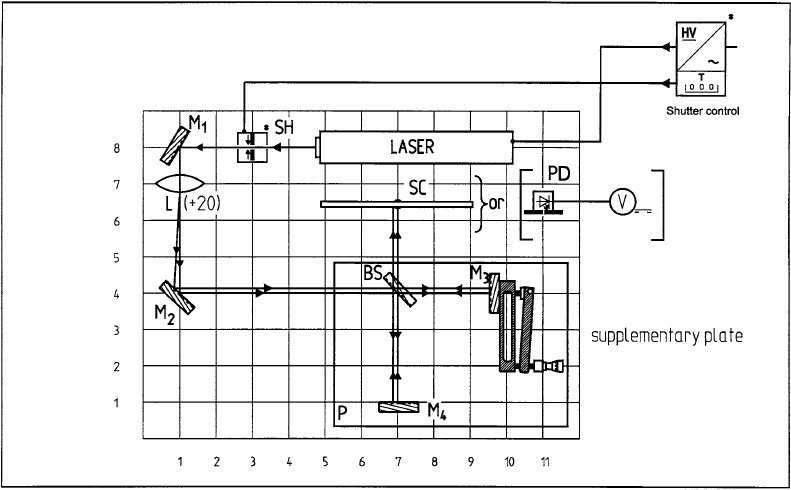
\includegraphics[width=\textwidth]{setup.png} % Replace with the actual path to your image
  \caption{Experimental setup of the Michelson Interferometer.\autocite{usm_2os3_manual}}
  \label{fig:michelson_setup}
\end{figure}

The Michelson Interferometer experiment \autocite{usm_2os3_manual} was conducted to determine the wavelength and coherence length of laser light. The interferometer was set up as shown in \autoref{fig:michelson_setup}, comprising components such as a He-Ne laser, mirrors, a beam splitter, and a screen, all mounted on an optical base plate. Initially, the lens \(L\) was removed to facilitate alignment, and the interferometer plate was positioned to align with the grid on the optical base. Mirrors \(M_1\) and \(M_2\) were placed along the fourth \(y\)-coordinate, and the beam splitter (\(BS\)) was temporarily removed. Mirror \(M_3\) was adjusted to ensure the laser beam returned to the same point on \(M_2\). Once aligned, the beam splitter was installed with its metallized side facing \(M_2\), splitting the beam into two paths. One path was directed toward \(M_3\), while the other was directed toward \(M_4\), aligned along the \(x\)-coordinate. The reflected beams from \(M_3\) and \(M_4\) were recombined to strike the same point on the screen (\(SC\)), and the lens \(L\) was inserted to produce a clear interference pattern.\\

To determine the laser light's wavelength, the optical path difference between \(M_3\) and \(BS\) was varied using a micrometer screw, with two complete turns corresponding to a displacement of \(1~\text{mm}\). The initial micrometer reading was recorded, and the micrometer screw was turned while counting the interference fringes passing a reference point on the screen. This procedure was repeated for fringe counts of \(30\), \(50\), and \(70\), with the final micrometer readings recorded for each trial. The wavelength \(\lambda\) was calculated using the formula:
\[
\lambda = \frac{2 \Delta d}{N}
\]
where \(\Delta d\) is the change in optical path length and \(N\) is the number of fringes counted. The results were compared with the known wavelength of the laser to evaluate the accuracy of the measurements.\\

To determine the coherence length, the screen (\(SC\)) was replaced with a photodiode (\(PD\)) aligned with the central fringe. The room was darkened to minimize noise and reduce the photodiode's dark current. The maximum (\(I_{\text{max}}\)) and minimum (\(I_{\text{min}}\)) fringe intensities were measured using a multimeter connected to the photodiode, and the measurements were optimized by adjusting the micrometer screw. Distances between mirrors \(M_3\), \(M_4\), and \(BS\) were recorded. The procedure was repeated for varying optical separations by moving \(M_4\) along the \(y\)-coordinate, changing the optical path difference between \(0\) and \(10~\text{cm}\). At larger separations, the radii of circular fringes decreased, reducing the accuracy of measurements for \(I_{\text{max}}\) and \(I_{\text{min}}\).\\

The coherence length was determined using two complementary methods: direct analysis of the experimental graph and theoretical modeling. First, the experimental contrast function (\(K\)) was calculated using the formula:
\[
K = \frac{I_{\text{max}} - I_{\text{min}}}{I_{\text{max}} + I_{\text{min}}}
\]
A graph of \(K\) versus the optical path difference (\(\Delta L\)) was plotted from the experimental data. The coherence length (\(L_{\text{coh}}\)) was identified as the optical path difference corresponding to the first x-intercept of the graph, where \(K\) reaches zero, indicating the disappearance of interference fringes.\\

In the second method, the theoretical contrast function was modeled using the equation:
\[
K = \left| \cos\left( \frac{\pi \Delta L}{L_{\text{coh}}} \right) \right|
\]
This model was fitted to the experimental data using numerical optimization techniques to minimize deviations. The fitted theoretical curve provided a refined estimate of the coherence length based on physics principles. Finally, the coherence lengths obtained from both methods were compared to ensure consistency and validate the experimental results.

\newpage
%%%%%%%%%%%%%%%%%%%%%%%%%%%%%%%%%%%%%%%%%%
\phantomsection
\section{\centering DATA ANALYSIS}
\label{sec:DATA ANALYSIS}
% Content for the DATA ANALYSIS section goes here.
\textbf{All data, calculation and programming python code of the experments are attached in the Appendices.}\\

\subsection{Michelson Interferometer Setup}

% Introduction to the Michelson Interferometer Setup
The Michelson interferometer is a precision optical instrument used to measure the coherence and phase shifts of light. It operates by splitting a coherent light source into two beams, directing them along different optical paths, and recombining them to produce an interference pattern. Below are the setup and resulting patterns observed during the experiment.\\

% Figure 1: The general setup of the Michelson interferometer
\begin{figure}[H]
    \centering
    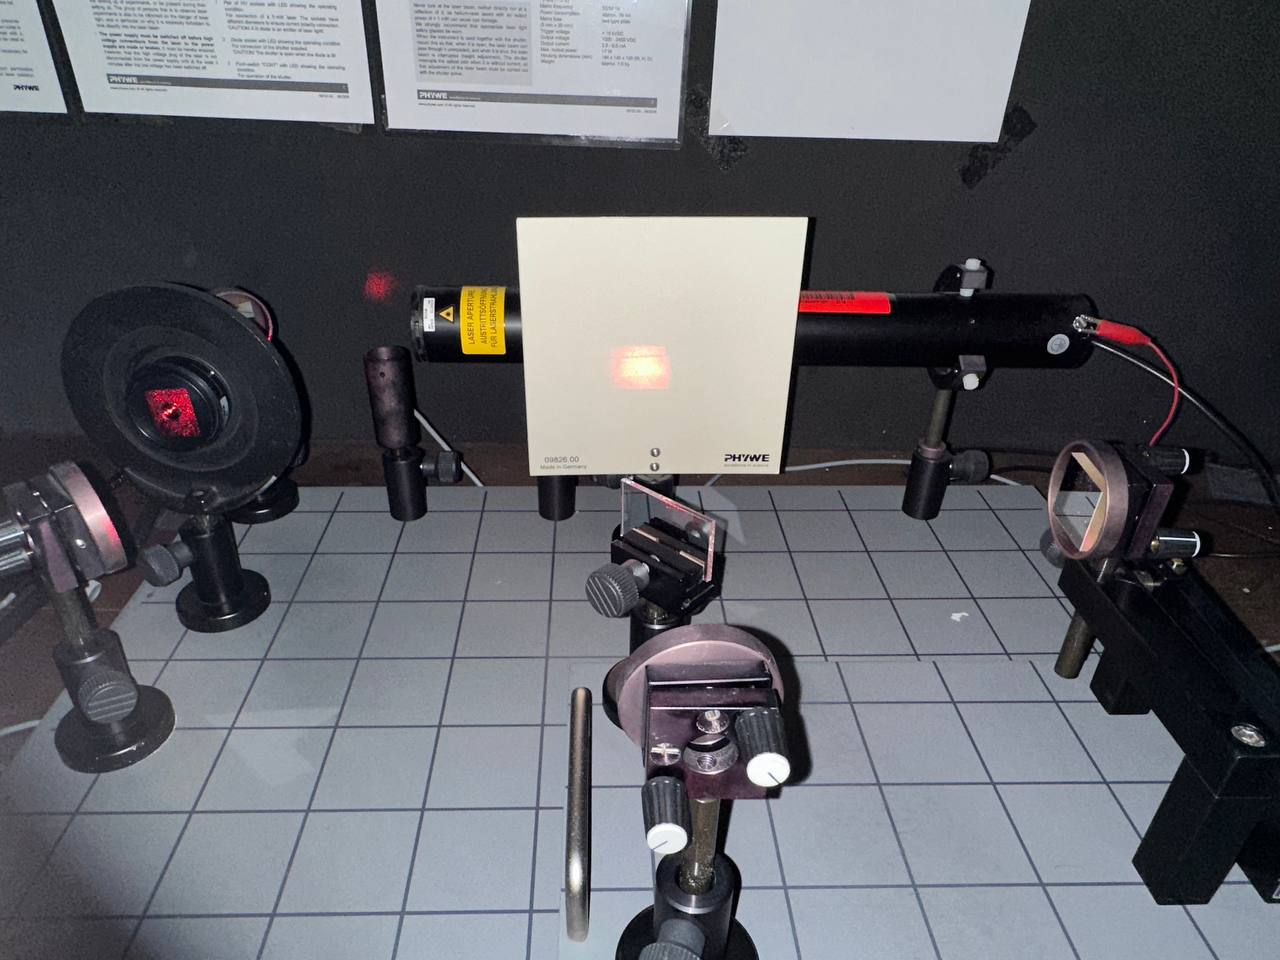
\includegraphics[width=0.6\textwidth]{image1.png} % Replace with the actual filename
    \caption{General setup of the Michelson interferometer, illustrating the placement of the laser source, beam splitter, mirrors, and observation screen. This configuration allows the generation of interference patterns as the optical paths are altered.}
    \label{fig:setup}
\end{figure}

% Introduction to observing the illuminated setup
Under laser illumination, the components of the Michelson interferometer produce a vivid display of the split and recombined light beams. This demonstrates the instrument's working principle.\\

% Figure 2: Illuminated setup with laser light
\begin{figure}[H]
    \centering
    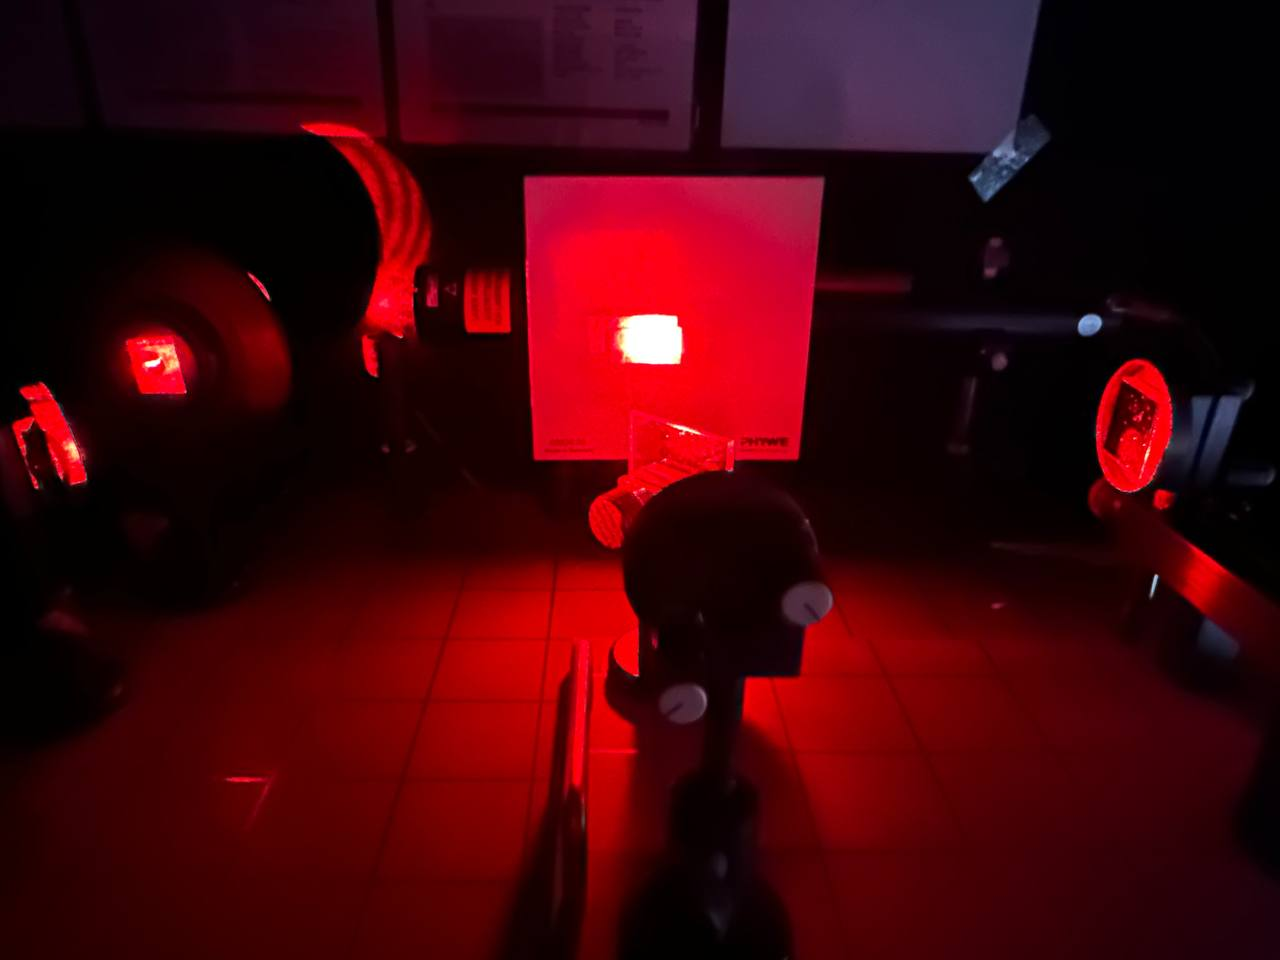
\includegraphics[width=0.6\textwidth]{image2.png} % Replace with the actual filename
    \caption{Illuminated setup of the Michelson interferometer under red laser light. The optical paths are clearly visible, demonstrating the interaction of light beams at various components such as the beam splitter and mirrors.}
    \label{fig:illuminated_setup}
\end{figure}

% Introduction to the interference fringes
When the optical path difference between the beams is within the coherence length, constructive and destructive interference produces the observed fringe patterns. These patterns are highly sensitive to changes in path length, making the Michelson interferometer ideal for precision measurements.\\

% Figure 3: Observed interference fringes
\begin{figure}[H]
    \centering
    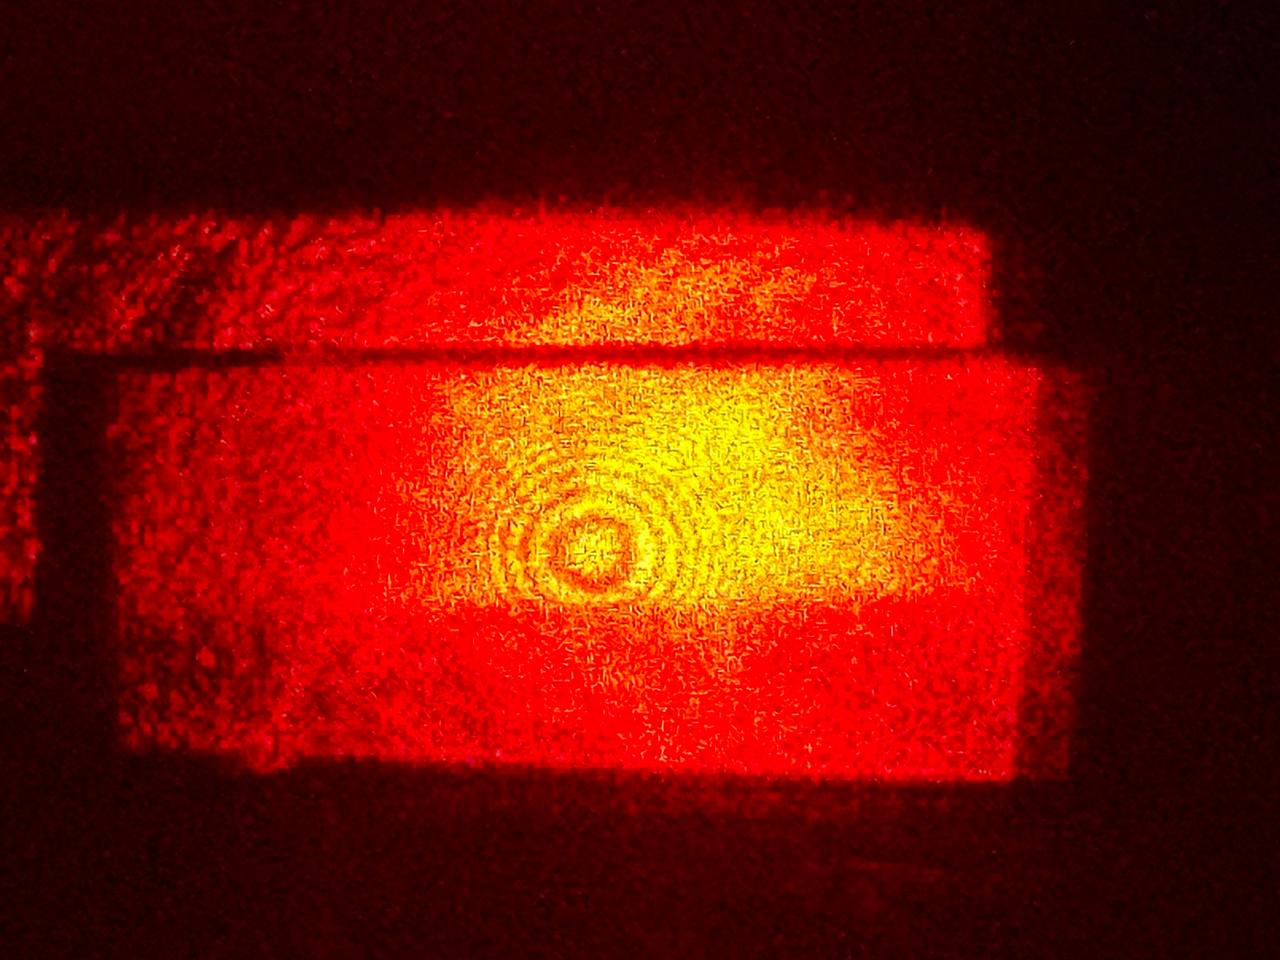
\includegraphics[width=0.6\textwidth]{image3.png} % Replace with the actual filename
    \caption{Interference fringes generated by the Michelson interferometer. The circular fringe pattern arises due to constructive and destructive interference as the optical path difference is altered.}
    \label{fig:fringes}
\end{figure}


\subsection{Wavelength Determination}

The \autoref{tab:results} summarizes the data for determining the wavelength of the laser light using the Michelson Interferometer.


\begin{table}[h!]
  \centering  
  \caption{Data for Wavelength Determination (Code: \autoref{Code: Wavelength Determination})}
  \begin{adjustbox}{width=\textwidth}
  \begin{tabular}{|c|p{3cm}|p{3cm}|c|c|c|c|c|}
  \hline
  \textbf{Count} & \multicolumn{2}{c|}{\textbf{Reference Position, ($d \pm 0.01$) mm}} & \textbf{Actual Position} & \textbf{Experimental Wavelength} & \textbf{Relative} & \textbf{Theoretical} & \textbf{Percentage} \\ 
  \cline{2-3}
   & \centering $d_i$ & \centering $d_f$ & $\Delta d$ ($\mu$m) & $\lambda_e$ (nm) & \textbf{Uncertainty} & $\lambda_0$ (nm) & \textbf{Discrepancy} \\
  \hline
  30 & \centering 1.00 & \centering 1.19 & $9.5 \pm 0.7$ & $633.33 \pm 47.14$ & 7.44\% & 632.8 & 0.08\% \\
  \hline
  50 & \centering 1.00 & \centering 1.32 & $16.0 \pm 0.7$ & $640.00 \pm 28.28$ & 4.42\% & 632.8 & 1.14\% \\
  \hline
  70 & \centering 1.00 & \centering 1.44 & $22.0 \pm 0.7$ & $628.57 \pm 20.20$ & 3.21\% & 632.8 & 0.67\% \\
  \hline
  \end{tabular}
  \end{adjustbox}
  \label{tab:results}
\end{table}

Based on \autoref{tab:results}, the calculated wavelength values are consistent across trials for different fringe counts ($N = 30, 50, 70$). The minor variation in $\lambda$ (ranging between 628.57 nm and 640.00 nm) is likely due to systematic errors such as minor misalignments, imperfections in the micrometer screw, or environmental factors like vibrations. The average wavelength across all trials is approximately 633.97 nm, which closely matches the expected value for the He-Ne laser of 632.8 nm \autocite{lielbeke_2015} \autocite{Thorlabs_HeNeLaser} , with the percentage of discrepancy of 0.18 \%. The results highlight the precision of the interferometer in measuring wavelengths, provided that alignment and fringe counting are performed with care. These observations validate the experimental setup and the accuracy of the measurements.\\

\subsection{Coherence Length Determination}
\indent

The \autoref{tab:coherence_length_grouped} demonstrates the relationship between the optical path different $\Delta L$ and the contrast function $K$.

\begin{table}[H]
  \centering
  \caption{Data for Coherence Length Determination (Sorted by Optical Path Difference) (Code: \autoref{code: Coherence Length Determination})}
  \label{tab:coherence_length_grouped}
  \resizebox{\textwidth}{!}{%
  \begin{tabular}{|c|c|c|p{3cm}|p{3cm}|c|}
      \hline
      \textbf{$M_4$ Position} & 
      \textbf{$M_3$ Position} & 
      \textbf{Optical Path Difference} & 
      \multicolumn{2}{c|}{\textbf{Voltage, ($V \pm 0.001$) V}} & 
      \textbf{Contrast Function} 
       \\ 
      \cline{4-5}
      \textbf{($X_{M_4} \pm 0.05$ cm)} & 
      \textbf{($X_{M_3} \pm 0.05$ cm)} & 
      \textbf{($\Delta L \pm 0.1$ cm)} & \centering \textbf{$V_{\text{max}}$} & \centering \textbf{$V_{\text{min}}$} & \textbf{$K \times 10^2$} \\ 
      \hline
      12.0 & 12.5 & 1.0 & \centering 0.325 & \centering 0.260 & 11.11 $\pm$ 0.05 \\ 
      \hline
      11.7 & 12.5 & 1.6 & \centering 0.360 & \centering 0.304 & 8.43 $\pm$ 0.04 \\ 
      \hline
      11.4 & 12.5 & 2.2 & \centering 0.348 & \centering 0.308 & 6.10 $\pm$ 0.03 \\ 
      \hline
      10.0 & 12.5 & 5.0 & \centering 0.370 & \centering 0.352 & 2.49 $\pm$ 0.01 \\ 
      \hline
      9.3 & 12.5 & 6.4 & \centering 0.356 & \centering 0.331 & 3.64 $\pm$ 0.02 \\ 
      \hline
      7.6 & 12.5 & 9.8 & \centering 0.360 & \centering 0.350 & 1.41 $\pm$ 0.01 \\ 
      \hline
  \end{tabular}%
  }
\end{table}

The data presented in \autoref{tab:coherence_length_grouped} demonstrates the relationship between the contrast function ($K$) and the optical path difference ($\Delta L$). At smaller optical path differences, such as $\Delta L = 1.0 \, \text{cm}$, the contrast function is relatively large ($K = 11.11 \pm 0.05$), indicating strong coherence between the interfering beams. This corresponds to a larger difference between the maximum voltage ($V_{\text{max}}$) and the minimum voltage ($V_{\text{min}}$), resulting in well-defined interference fringes.\\

As the optical path difference increases, $K$ decreases significantly. For example, at $\Delta L = 6.4 \, \text{cm}$, $K = 3.64 \pm 0.02$, and at $\Delta L = 9.8 \, \text{cm}$, $K = 1.41 \pm 0.01$. This trend indicates weaker coherence between the interfering beams as the optical path difference increases, leading to diminished fringe visibility. The smaller difference between $V_{\text{max}}$ and $V_{\text{min}}$ observed in the data supports this interpretation.\\


\begin{figure}[H]
    \centering
    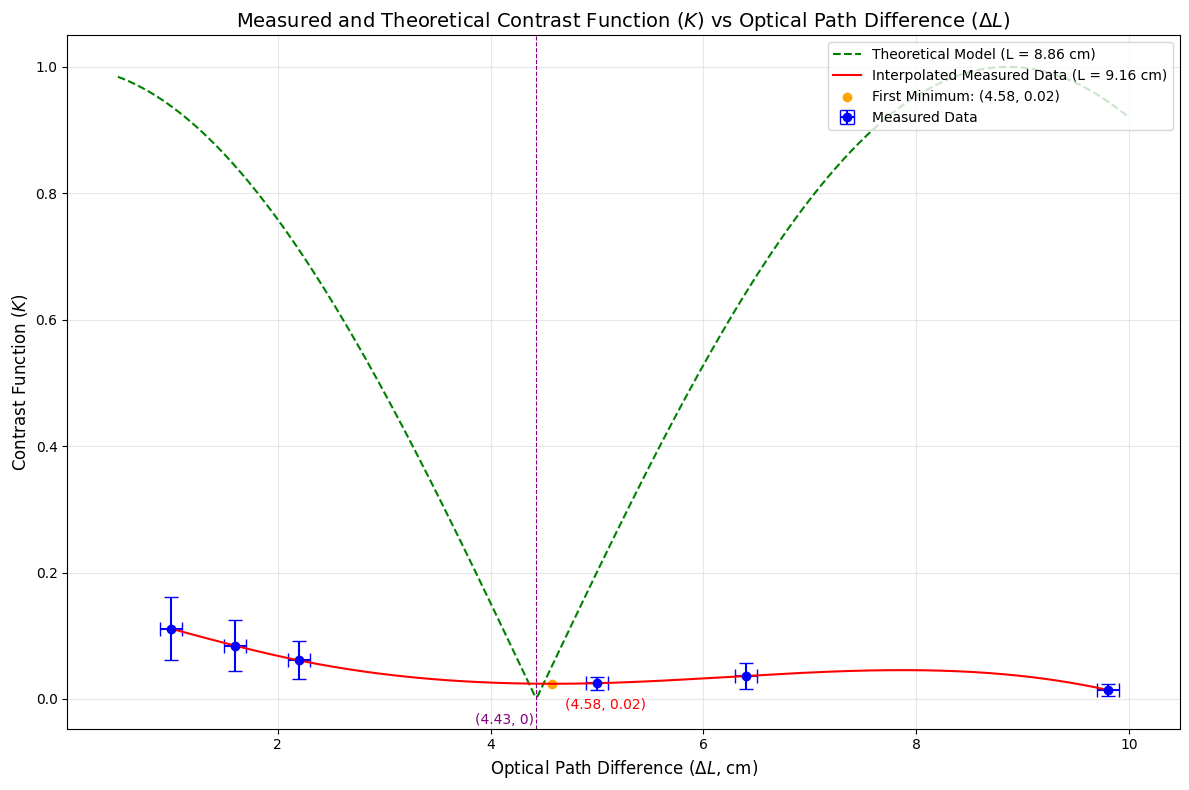
\includegraphics[width=0.9\textwidth]{image4.png}
    \caption{Measured and theoretical contrast function (\( K \)) as a function of optical path difference (\( \Delta L \)). The theoretical model (green dashed line) is based on the coherence length \( L = 8.86 \, \text{cm} \), while the interpolated curve of the measured data (red line) suggests a coherence length \( L = 9.16 \, \text{cm} \). The first minimum point in the measured data and the first x-intercept of the theoretical model are labeled. (Code: \autoref{code: Graphical representation of the contrast function})}
    \label{fig:contrast_function}
\end{figure}

The graph in Figure~\ref{fig:contrast_function} illustrates the variation in the contrast function (\( K \)) as a function of the optical path difference (\( \Delta L \)). The green dashed line in Figure~\ref{fig:contrast_function} represents the theoretical model for the contrast function \( K \), which is governed by the formula:
\[
K = \left| \cos\left(\frac{\pi \Delta L}{L}\right) \right|,\\
\]
where \( \Delta L \) is the optical path difference and \( L \) is the coherence length of the light source. In this model, the coherence length \( L \) is calculated based on the position of the first x-intercept of the curve. The first x-intercept occurs where \( K = 0 \), corresponding to the first destructive interference point. This happens at \( \Delta L = 4.43 \, \text{cm} \), which is highlighted in the graph with a purple dashed line. Using this position, the coherence length \( L \) is calculated as:
\[
L = \frac{2 \cdot \Delta L}{(2n + 1)} \quad \text{for} \, n = 0,
\]
yielding \( L = 8.86 \, \text{cm} \).\\

The theoretical model predicts periodic behavior of the contrast function as \( \Delta L \) increases, with repeated x-intercepts corresponding to higher-order destructive interference points. The periodic nature of the cosine-based model reflects the coherence properties of the light source, as \( K \) alternates between maxima and zero values due to constructive and destructive interference. The position of the first x-intercept is crucial because it allows for an accurate determination of \( L \), which is a fundamental parameter characterizing the light source's coherence.\\

The experimental data, represented by blue markers with error bars, include uncertainties in both \( K \) and \( \Delta L \). The red curve is the cubic interpolation of the measured data, which smoothens the experimental results and provides a clearer visualization of the trend. The orange marker indicates the first minimum of the interpolated curve at \( \Delta L = 4.58 \, \text{cm} \), where the contrast function exhibits a notable drop. This minimum corresponds to the point where the interference intensity decreases significantly, reflecting a reduction in coherence. The coherence length is determined from this minimum using \( L = 2 \cdot \Delta L_{\text{min}} \), aligning with theoretical expectations. The interpolated curve suggests a coherence length of \( L = 9.16 \, \text{cm} \), slightly higher than the theoretical prediction.\\

The coherence length (\( L \)) of the light source was determined both theoretically and experimentally. The theoretical coherence length was calculated as \( L_{\text{theoretical}} = 8.86 \, \text{cm} \), based on the position of the first x-intercept at \( \Delta L = 4.43 \, \text{cm} \). Experimentally, the coherence length was derived from the first minimum of the interpolated measured data, resulting in \( L_{\text{measured}} = 9.16 \, \text{cm} \), with the first minimum point observed at \( \Delta L_{\text{min}} = 4.58 \, \text{cm} \).\\

The percentage difference between the theoretical and measured coherence lengths was found to be 3.33\% (Code: \autoref{code: Percentage Difference Calculation}). This small difference demonstrates good agreement between the theoretical model and the experimental results, confirming the reliability of the theoretical cosine-based formula used to describe the contrast function (\( K \)).\\

The agreement between the measured data and the theoretical model reinforces the validity of using this cosine-based function to describe the interference pattern. The first x-intercept provides a precise reference for calculating \( L \), while subsequent x-intercepts confirm the periodicity expected in coherent light interference. Minor deviations observed in the measured data, compared to the theoretical model, are likely due to real-world experimental limitations such as alignment errors or detector imperfections.\\




\newpage
%%%%%%%%%%%%%%%%%%%%%%%%%%%%%%%%%%%%%%%%%
\phantomsection
\section{\centering DISCUSSION}
\label{sec:DISCUSSION}
% Content for the DISCUSSION section goes here.
\indent

The Michelson Interferometer was set up to split a coherent laser beam into two perpendicular paths, reflect them off mirrors, and recombine them to produce interference patterns. The experimental setup required precise alignment of the beam splitter, mirrors, and optical components to ensure that the two beams recombined accurately. The resulting interference patterns, observed on the screen, appeared as circular fringes due to constructive and destructive interference. At smaller optical path differences ($\Delta L$), the fringes were distinct and highly visible, indicating strong coherence between the two beams. As $\Delta L$ increased, the visibility of the fringes diminished, reflecting a reduction in coherence. This behavior provided an intuitive demonstration of the principles of interference and coherence.\\

For wavelength determination, the optical path difference ($\Delta L$) was systematically varied using a micrometer screw, and the number of fringes ($N$) passing a reference point was counted. The calculated wavelengths for $N = 30, 50, 70$ ranged from $628.57 \, \text{nm}$ to $640.00 \, \text{nm}$, with an average value of $633.97 \, \text{nm}$. This result closely matches the theoretical wavelength of $632.8 \, \text{nm}$, with a minimal percentage discrepancy of $0.18\%$. The small variations between trials were likely caused by minor misalignments, imperfections in the micrometer screw, and environmental factors such as vibrations. Despite these challenges, the results highlight the precision and reliability of the Michelson Interferometer in measuring wavelengths.\\

In determining the coherence length, the contrast function ($K$) was plotted as a function of $\Delta L$. The data showed that $K$ decreased steadily with increasing $\Delta L$, indicating reduced coherence as the optical path difference approached the coherence length. The theoretical contrast function is described by:
\[
K = \left| \cos \left( \frac{\pi \Delta L}{L_{\text{coh}}} \right) \right|,\\
\]

where $L_{\text{coh}}$ is the coherence length. The first x-intercept of the theoretical curve, which corresponds to $K = 0$, was observed at $\Delta L_{\text{theoretical}} = 4.43 \, \text{cm}$. This value gives a theoretical coherence length of $L_{\text{theoretical}} = 8.86 \, \text{cm}$. From the experimental data, the first minimum of the interpolated curve occurred at $\Delta L_{\text{measured}} = 4.58 \, \text{cm}$, yielding a measured coherence length of $L_{\text{measured}} = 9.16 \, \text{cm}$. The percentage difference between the theoretical and experimental coherence lengths was $3.33\%$, indicating good agreement between the two values. The consistency between the theoretical model and experimental data validates the use of the Michelson Interferometer for coherence analysis.\\

The  \autoref{fig:contrast_function} with graph of $K$ versus $\Delta L$ showed a periodic behavior predicted by the cosine-based theoretical model, with subsequent x-intercepts representing higher-order destructive interference points. The experimental data closely followed this trend, with minor deviations due to alignment errors, detector sensitivity, and reduced fringe visibility at larger $\Delta L$. These deviations were minimal and did not significantly affect the accuracy of the results.\\

Precautionary steps were taken to ensure laser safety during the experiment, protecting both the experimenters and the equipment. The laser beam was aligned at a low height to prevent accidental exposure to the eyes, and appropriate laser safety goggles were worn throughout the experiment. The experiment was conducted in a closed and controlled environment to minimize exposure to reflections or scattered beams, and the laser beam paths were clearly marked to reduce risks of accidental interference.\\

Despite the overall success, several errors may have affected the experiment's accuracy. Slight misalignments of the mirrors, beam splitter, or photodetector could have distorted the interference patterns and reduced measurement accuracy. These alignment errors can be mitigated by using fine adjustment screws and verifying alignment with an alignment laser. Environmental vibrations, such as those from nearby equipment or human movement, may have introduced noise and caused fluctuations in the fringe patterns. Placing the interferometer on an anti-vibration table (Optical table) and isolating it from disturbances can address this issue. The photodiode’s sensitivity may have introduced noise, particularly at larger optical path differences where fringe visibility was low. A more sensitive detector with lower noise levels could improve accuracy. Manual fringe counting also introduced potential for human error, which could be eliminated by employing an automated fringe-counting system with image processing.\\

To improve the reliability and accuracy of the experiment, integrating an automated system for recording micrometer readings, fringe counts, and photodiode voltages would reduce human error. Using higher-precision optical components and conducting the experiment in a controlled environment to minimize temperature and pressure variations would further enhance accuracy. Advanced computational methods could also be employed to analyze fringe patterns and contrast functions, allowing better fitting of experimental data to theoretical models.\\

This experiment opens avenues for further exploration. Future studies could involve inserting transparent materials into one arm of the interferometer to measure their refractive indices by analyzing shifts in the interference fringes. Broadband light sources, such as LEDs, could be used to investigate coherence properties and compare them to narrowband lasers. Advanced applications of the Michelson Interferometer in precision metrology, such as detecting gravitational waves \autocite{michelson_interferometer_wikipedia} or measuring nanometer-scale displacements, could also be explored. Phase-shifting interferometry and quantum interference studies, such as single-photon interference experiments, are additional directions for further research. These possibilities highlight the versatility and importance of the Michelson Interferometer in advancing optical physics.


\newpage
%%%%%%%%%%%%%%%%%%%%%%%%%%%%%%%%%%%%%%%%%%
\phantomsection
\section{\centering CONCLUSION}
\label{sec:CONCLUSION}
% Content for the CONCLUSION section goes here.
\indent 

The Michelson Interferometer experiment produced results consistent with theoretical predictions. The measured wavelength of the He-Ne laser was \( 633.97 \, \text{nm} \), closely matching the theoretical value of \( 632.8 \, \text{nm} \) with a \( 0.18\% \) percentage discrepancy. The coherence length was determined to be \( 9.16 \, \text{cm} \), aligning well with the theoretical value of \( 8.86 \, \text{cm} \) and showing a \( 3.33\% \) percentage difference. These outcomes confirm the accuracy and reliability of the Michelson Interferometer for optical measurements.

\newpage
%%%%%%%%%%%%%%%%%%%%%%%%%%%%%%%%%%%%%%%%%%
\phantomsection
\section{\centering REFERENCES}
\label{sec:REFERENCES}

\printbibliography[heading=none]

\newpage
%%%%%%%%%%%%%%%%%%%%%%%%%%%%%%%%%%%%%%%%%%
\phantomsection
\section{\centering APPENDICES}
\label{sec:APPENDICES}

%Code
\subsection{Calculation for wavelength determination}
\begin{lstlisting}[language=Python]
  import numpy as np
  import pandas as pd
  
  # Input data
  counts = np.array([30, 50, 70])
  initial_readings = np.array([1.00, 1.00, 1.00])  # in mm
  final_readings = np.array([1.19, 1.32, 1.44])    # in mm
  
  theoretical_wavelength = 632.8  # in nm
  uncertainty_position = 0.01      # in mm
  
  def calculate_data(counts, initial_readings, final_readings, theoretical_wavelength, uncertainty_position):
      # Calculate actual position change in micrometers (um)
      delta_d = ((final_readings - initial_readings) * 1000) / 20  # Convert mm to um and divide by 20
  
      # Uncertainty in delta_d (same as uncertainty in position, converted to um)
      uncertainty_delta_d = np.sqrt(2 * ((uncertainty_position * 1000) / 20)**2)
  
      # Calculate experimental wavelength (in nm)
      lambda_e = 2 * delta_d / counts * 1000
  
      # Uncertainty in wavelength (propagated)
      uncertainty_lambda = lambda_e * (uncertainty_delta_d / delta_d)
  
      # Relative uncertainty in percentage
      relative_uncertainty = (uncertainty_lambda / lambda_e) * 100
  
      # Percentage discrepancy
      percentage_discrepancy = np.abs(lambda_e - theoretical_wavelength) / theoretical_wavelength * 100
  
      # Mean wavelength and mean percentage discrepancy
      mean_wavelength = np.mean(lambda_e)
      mean_percentage_discrepancy = percentage_discrepancy = np.abs(mean_wavelength - theoretical_wavelength) / theoretical_wavelength * 100
  
      # Prepare data for table
      data = {
    "Count ($N$)": counts,
    "Initial Position (mm)": initial_readings,
    "Final Position (mm)": final_readings,
    "Actual Position Change ($\Delta d$, $\mu$m)": delta_d,
    "Uncertainty in $\Delta d$ ($\mu$m)": uncertainty_delta_d,
    "Experimental Wavelength ($\lambda_e$, nm)": lambda_e,
    "Uncertainty in $\lambda_e$ (nm)": uncertainty_lambda,
    "Relative Uncertainty (\%)": relative_uncertainty,
    "Theoretical Wavelength ($\lambda_0$, nm)": [theoretical_wavelength] * len(counts),
    "Percentage Discrepancy (\%)": percentage_discrepancy
    }

  
      return pd.DataFrame(data), mean_wavelength, mean_percentage_discrepancy
  
  # Generate the table and calculations
  data_table, mean_wavelength, mean_percentage_discrepancy = calculate_data(
      counts, initial_readings, final_readings, theoretical_wavelength, uncertainty_position
  )
  
  # Display the rounded table
  data_table_rounded = data_table.round(2)
  
  # Save or print the table
  data_table_rounded.to_csv("experimental_data_table.csv", index=False)  # Save as CSV
  print(data_table_rounded)  # Print the table
  
  # Print the results
  print("Mean Experimental Wavelength (nm):", round(mean_wavelength, 2))
  print("Percentage Discrepancy (%):", round(mean_percentage_discrepancy, 2))  
\end{lstlisting}
\label{Code: Wavelength Determination}
\newpage
\subsubsection*{Output}
\begin{lstlisting}[language=Python]
  Count (N)  Initial Position (mm)  Final Position (mm)  \
  0         30                    1.0                 1.19   
  1         50                    1.0                 1.32   
  2         70                    1.0                 1.44   
  
     Actual Position Change ($\Delta d, \mu m$)  Uncertainty in $$\Delta d$$ ($\mu m$)  \
  0                              9.5                    0.71   
  1                             16.0                    0.71   
  2                             22.0                    0.71   
  
     Experimental Wavelength ($\lambda_e, nm$)  Uncertainty in $\lambda_e$($nm$)  \
  0                             633.33                    47.14   
  1                             640.00                    28.28   
  2                             628.57                    20.20   
  
     Relative Uncertainty ($\%$)  Theoretical Wavelength ($\lambda_0, nm$)  \
  0                      7.44                             632.8   
  1                      4.42                             632.8   
  2                      3.21                             632.8   
  
     Percentage Discrepancy ($\%$)  
  0                        0.18  
  1                        0.18  
  2                        0.18  
  Mean Experimental Wavelength ($nm$): 633.97
  Percentage Discrepancy ($\%$): 0.18

\end{lstlisting}
\newpage
%%%
\subsection{Calculation for coherence length determination}
\begin{lstlisting}[language=Python]
  import pandas as pd
  import numpy as np
  
  # Input data
  data = {
      "M4 Position (cm)": [7.6, 9.3, 10.0, 11.4, 11.7, 12.0],
      "M3 Position (cm)": [12.5, 12.5, 12.5, 12.5, 12.5, 12.5],
      "Maximum Intensity (Imax $\pm$ 0.001 V)": [0.360, 0.356, 0.370, 0.348, 0.360, 0.325],
      "Minimum Intensity (Imin $\pm$ 0.001 V)": [0.350, 0.331, 0.352, 0.308, 0.304, 0.260]
  }
  
  # Convert to DataFrame
  df = pd.DataFrame(data)
  
  # Calculate optical path difference ($\Delta L$)
  df["Optical Path Difference ($\Delta L$, cm)"] = (df["M3 Position (cm)"] - df["M4 Position (cm)"]) * 2
  
  # Define uncertainties
  Imax_error = 0.001  # Error in Imax
  Imin_error = 0.001  # Error in Imin
  
  # Calculate Contrast Function (K)
  df["Contrast Function (K)"] = (
      (df["Maximum Intensity (Imax $\pm$ 0.001 V)"] - df["Minimum Intensity (Imin $\pm$ 0.001 V)"]) /
      (df["Maximum Intensity (Imax $\pm$ 0.001 V)"] + df["Minimum Intensity (Imin $\pm$ 0.001 V)"])
  )
  
  # Calculate Uncertainty of K using error propagation
  df["Uncertainty of K"] = df["Contrast Function (K)"] * np.sqrt(
      (Imax_error / df["Maximum Intensity (Imax $\pm$ 0.001 V)"])**2 +
      (Imin_error / df["Minimum Intensity (Imin $\pm$ 0.001 V)"])**2
  )
  
  # Round results for better readability
  df_rounded = df.round(4)
  
  # Display the DataFrame
  import ace_tools as tools; tools.display_dataframe_to_user(name="Optical Path Difference and Contrast Analysis", dataframe=df_rounded)  
\end{lstlisting}
\label{code: Coherence Length Determination}
\subsubsection*{Output}
\begin{lstlisting}[language=Python]
  M4 Position (cm)  M3 Position (cm)  Maximum Intensity (Imax  $\pm$ 0.001 V)  \
  0               7.6              12.5                               0.360   
  1               9.3              12.5                               0.356   
  2              10.0              12.5                               0.370   
  3              11.4              12.5                               0.348   
  4              11.7              12.5                               0.360   
  5              12.0              12.5                               0.325   
  
     Minimum Intensity (Imin  $\pm$ 0.001 V)  Optical Path Difference ($\Delta L$, cm)  \
  0                               0.350                               9.8   
  1                               0.331                               6.4   
  2                               0.352                               5.0   
  3                               0.308                               2.2   
  4                               0.304                               1.6   
  5                               0.260                               1.0   
  
     Contrast Function (K)  Uncertainty of K  
  0                 0.0141            0.0001  
  1                 0.0364            0.0002  
  2                 0.0249            0.0001  
  3                 0.0610            0.0003  
  4                 0.0843            0.0004  
  5                 0.1111            0.0005
\end{lstlisting}
\newpage
%%%
\subsection{Graphical representation of the contrast function}
\begin{lstlisting}[language=Python]
  import matplotlib.pyplot as plt
  import numpy as np
  from scipy.interpolate import interp1d
  from scipy.signal import argrelextrema
  
  # Data
  delta_L = np.array([1.0, 1.6, 2.2, 5.0, 6.4, 9.8])  # Optical path difference (d, cm)
  K = np.array([11.11, 8.43, 6.10, 2.49, 3.64, 1.41]) / 100  # Contrast Function (K), scaled to proper range
  K_error = np.array([0.05, 0.04, 0.03, 0.01, 0.02, 0.01])  # Uncertainty of K
  delta_L_error = np.full_like(delta_L, 0.1)  # Error in optical path difference (0.1 cm)
  
  # Theoretical coherence length
  L_theoretical = np.mean(np.pi * delta_L / np.arccos(K))  # Approximate L from the given data
  
  # Generate delta_L values for the theoretical curve
  delta_L_theoretical = np.linspace(0.5, 10, 500)  # Fine-grained d values for the curve
  K_theoretical = np.abs(np.cos(np.pi * delta_L_theoretical / L_theoretical))  # Calculate theoretical K
  
  # Interpolation of measured data for smooth curve
  interp_function = interp1d(delta_L, K, kind='cubic')  # Cubic interpolation
  delta_L_smooth = np.linspace(min(delta_L), max(delta_L), 500)  # Smooth d values
  K_smooth = interp_function(delta_L_smooth)  # Interpolated K values
  
  # Find the first x-intercept for the theoretical model
  x_intercepts = [(2 * n + 1) * L_theoretical / 2 for n in range(int(max(delta_L_theoretical) / (L_theoretical / 2)))]
  first_x_intercept = x_intercepts[0]
  
  # Find the local minima in the interpolated curve
  min_indices = argrelextrema(K_smooth, np.less)[0]
  first_min_index = min_indices[0]
  first_min_delta_L = delta_L_smooth[first_min_index]
  first_min_K = K_smooth[first_min_index]
  L_coherence = 2*first_min_delta_L
  
  # Plotting
  plt.figure(figsize=(12, 8))
  
  # Measured data with horizontal and vertical error bars
  plt.errorbar(delta_L, K, xerr=delta_L_error, yerr=K_error, fmt='o', color='blue', capsize=5, label='Measured Data')
  
  # Theoretical model
  plt.plot(delta_L_theoretical, K_theoretical, color='green', linestyle='--', label=f'Theoretical Model (L = {L_theoretical:.2f} cm)')
  
  # Interpolated measured data
  plt.plot(delta_L_smooth, K_smooth, color='red', linestyle='-', label=f'Interpolated Measured Data (L = {L_coherence:.2f} cm)')
  
  # Highlight the first x-intercept for the theoretical model
  plt.axvline(first_x_intercept, color='purple', linestyle='--', linewidth=0.8)
  plt.text(first_x_intercept - 0.3, -0.04, f'({first_x_intercept:.2f}, 0)', color='purple', fontsize=10, ha='center')
  
  # Highlight the first minimum point and label its coordinates
  plt.scatter(first_min_delta_L, first_min_K, color='orange', label=f'First Minimum: ({first_min_delta_L:.2f}, {first_min_K:.2f})')
  plt.text(first_min_delta_L + 0.5, first_min_K - 0.04, f'({first_min_delta_L:.2f}, {first_min_K:.2f})', 
           color='red', fontsize=10, ha='center')
  
  # Labels, title, and legend
  plt.title("Measured and Theoretical Contrast Function ($K$) vs Optical Path Difference ($\Delta L$)", fontsize=14)
  plt.xlabel("Optical Path Difference ($\Delta L$, cm)", fontsize=12)
  plt.ylabel("Contrast Function ($K$)", fontsize=12)
  plt.grid(alpha=0.3)
  plt.legend(fontsize=10, loc='upper right')
  plt.tight_layout()
  
  # Show plot
  plt.show()
  
  # Print results for verification
  print(f"First X-Intercept (Theoretical): ({first_x_intercept:.2f}, 0)")
  print(f"First Minimum Point (Measured): ({first_min_delta_L:.2f}, {first_min_K:.2f})")  
\end{lstlisting}
\label{code: Graphical representation of the contrast function}

\subsubsection*{Output}

\begin{figure}[H]
  \centering
  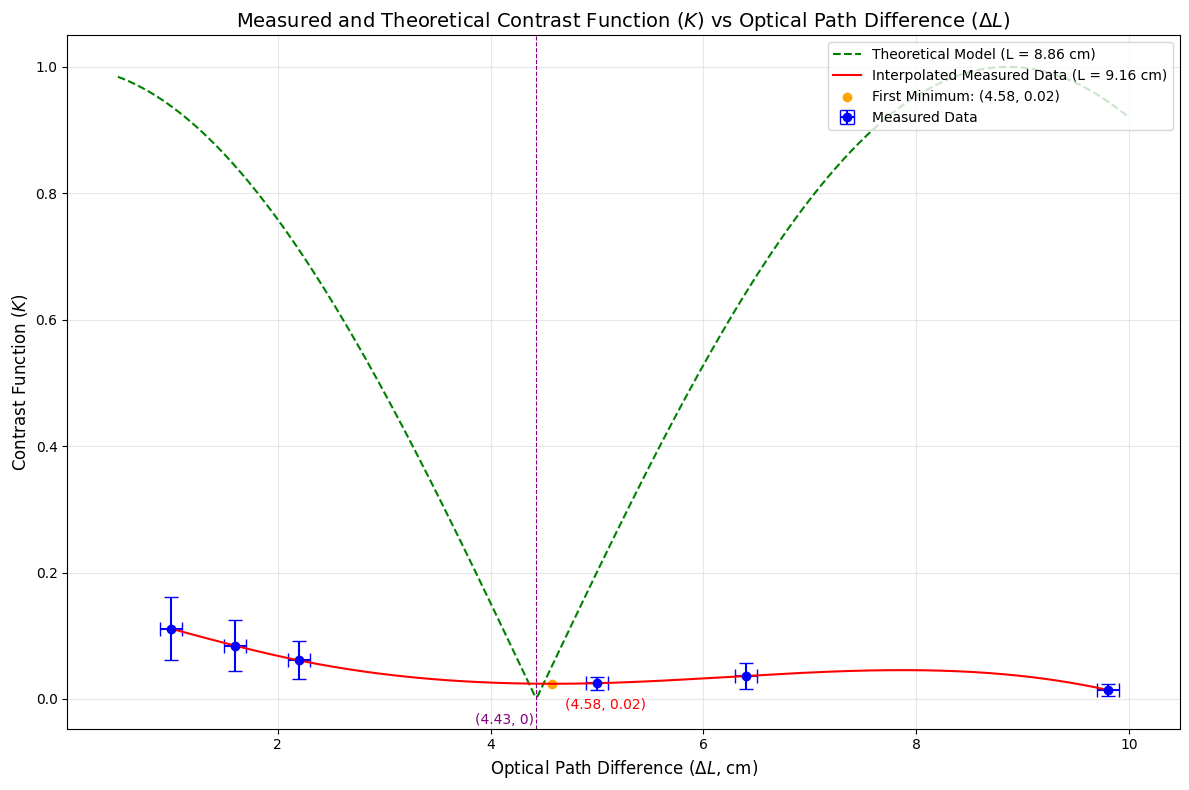
\includegraphics[width=\textwidth]{image4.png}
\end{figure}

\begin{lstlisting}[language=Python]
  First X-Intercept (Theoretical): (4.43, 0)
  First Minimum Point (Measured): (4.58, 0.02)  
\end{lstlisting}
\newpage
%%%
\subsection{Calculation for percentage difference}
\begin{lstlisting}[language=Python]
  def calculate_percentage_difference(value1, value2):
  """
  Calculate the percentage difference between two values.

  Parameters:
  value1 (float): The first value (e.g., theoretical coherence length).
  value2 (float): The second value (e.g., measured coherence length).

  Returns:
  float: The percentage difference between the two values.
  """
  # Calculate percentage difference based on the formula
  percentage_difference = 100 * abs(value1 - value2) / ((value1 + value2) / 2)
  return percentage_difference

# Values from the provided image
theoretical_length = 8.86  # Theoretical coherence length in cm
measured_length = 9.16     # Measured coherence length in cm

# Calculate the percentage difference
result = calculate_percentage_difference(theoretical_length, measured_length)

# Display the result
print(f"The percentage difference is {result:.2f}%.")

\end{lstlisting}
\label{code: Percentage Difference Calculation}

\subsubsection*{Output}
\begin{lstlisting}[language=Python]
The percentage difference is 3.33%.
\end{lstlisting}

\end{document}
